%!TEX root = ../main.tex
With the study of topology we can obtain many useful tools to develop our theory. First we will define the notion of metrical space and we will compare it with the notion of topological spaces.
\subsubsection{Metric spaces}

First we need to deal with the concept of distance: we have to obtain an abstract tool to quantify how close are two elements of the same set:
\begin{defn}
	Let $X$ be a non-empty set.\\
	A function $d:\, X\times X \to \left[0,+\infty\right)$ is called \emph{distance} or \emph{metric} on $X$ if $\forall x,y,z \in X$ these properties hold:
	\begin{itemize}
		\item \emph{non-negativity}:																
		$$d(x,y)\geq0;$$
		\item \emph{identity of indiscernibles}:\footnotemark{}
		$$d(x,y)=0 \iff y=x;$$
		\item \emph{symmetry}:																		
		$$d(x,y)=d(y,x);$$
		\item \emph{triangle inequality or subadditivity}:											
		$$d(x,y) \leq d(x, z) + d(z, y).$$
	\end{itemize}
\end{defn}
\footnotetext{\itatrasl{annullamento}}
Observe that for this definition we had no need of an algebraic structure on $X$. It is possible to define multiple distances on the same set. Here we present some broadly-used distances. 
\begin{exam}
	On a generic non-empty set $X$ we can define the \emph{discrete distance}  as follows:
	$$ 
		d\left(x,y\right) = 
		\begin{cases}
			0 & \text{if } x = y \\
			1 & \text{if } x \neq y
		\end{cases}
	.
	$$
\end{exam}
\begin{exam}
	On $\RR^N$ we can define the \emph{euclidean distance}:
	$$d_e(x,y) =\sqrt{\sum_{i=1}^{n}(x_i-y_i)^2}$$
	which is a particular case of the following ($p=2$):
	$$d_p(x,y) = \left(\sum_{i=1}^{n}|x_i-y_i|^p\right)^\frac 1 p.$$
	For exercise check that $d_e$ is a distance.\footnotemark{}
\end{exam}
\begin{exam}
	From the previous formula, with particular values of $p$, other metric can be defined:
	$$
		d_1(x,y) 
		= \sum_{i=1}^{n}|x_i-y_i|, 
		\quad d_\infty(x,y) 
		= \max_{i=1, \ldots, n}|x_i-y_i|
	.
	$$
\end{exam}
\footnotetext{Use Cauchy--Schwarz inequality: $\sum_{k=1}^{n}|a_kb_k|\leq\left(\sum_{k=1}^{n}a_k^2\right)^\frac 1 2 \left(\sum_{k=1}^{n}b_k^2\right)^\frac 1 2$}


Considering a set with a metric we get a powerful environment on which we can build useful tools:
\begin{defn}
	If $d$ is a distance on $X \neq \varnothing$, then the couple $\left(X,d\right)$ is called \emph{metric space}.
\end{defn} 

\paragraph{Open balls} or spherical neighbourhood are the sets that contain all points which are ``close'' from a given point. The geometry of those balls depends on the metric considered.
\begin{defn}
	Let $\left(X,d\right)$ a metric space, $x_0 \in X$ and $r>0$.\\
	The \emph{open ball} or \emph{spherical neighbourhood} of center $x_0$ and radius $r$ is defined as:
	$$ B_d \left( x_0,r \right) \coloneqq \{ x \in X : d\left(x,x_0\right) < r \} $$
\end{defn}

Clearly different distances will produce differently shaped balls in $\RR^N$ (see figure \vref{balls-different-metrics}):

\begin{figure}[H]
	\centering
	% Unit circle plot style
	\pgfplotsset{unit circle/.style={width=4cm,height=4cm,axis lines=middle,xtick=\empty,ytick=\empty,axis equal,enlargelimits,xmax=1,ymax=1,xmin=-1,ymin=-1,domain=0:pi/2}}
	\begin{tikzpicture}
	\coordinate (prev); % Store previous plot position
	\foreach \p / \t in {4/\frac{1}{2}, 2/1, 1/2, 0.0001/\infty} { % Loop through the plots to draw
	    % \p is the exponent in the function to plot
	    % \t is the p parameter to print
	    \begin{axis}[at={(prev)},unit circle,anchor=west]
	        \foreach \ss in {1,-1} {
		        \foreach \cs in {1,-1} {
		            \addplot[] ({\cs*(cos(deg(x)))^\p},{\ss*(sin(deg(x))^\p});
		        }
	        }
	    \end{axis}
	    \node[below=0.5cm, anchor=base] at (current axis.south) {$p=\t$}; % Print p
	    \coordinate[right=0.5cm] (prev) at (current axis.east) ; % Set position for next plot
	}
	\end{tikzpicture}
	\caption{balls in different distances on $\RR^2$}
	\label{balls-different-metrics}
\end{figure}

\begin{exam}
	Let $d$ be the discrete metric on $X$. Then we have:
	$$
		B_d\left(x_0,r\right) = 
		\begin{cases}
			\{x_0\} & \text{if } r \leq 1 \\
			X & \text{if } r >1
		\end{cases}
	.
	$$
\end{exam}

\paragraph{On function spaces} distances and neighborhoods can be defined, consider $X=\Cc^0\left(\left[a,b\right]\right)$ and these two possible distances:
$$
	d_1\left(f,g\right) 
	\coloneqq \int_{a}^{b}|f\left(x\right)-g\left(x\right)|\dx, 
	\qquad d_\infty\left(f,g\right) 
	\coloneqq \max_{x\in\left[a,b\right]}|f\left(x\right)-g\left(x\right)|
.
$$

These two metrics generate very different neighborhoods (see figure \vref{spherical-nbh-Cc0-different-distances}):
\begin{itemize}
	\item $B_{d_1\left(f, r\right)}$ is the set of functions in $X$ subject to $\int_a^b |f-g| < r$;
	\item $B_{d_\infty\left(f, r\right)}$ is instead the set of functions in $X$ whose graphs is contained in a ``strip'' around $f$.
\end{itemize}

\begin{figure}[h]
	\centering
	\begin{subfigure}[b]{.4\linewidth}
		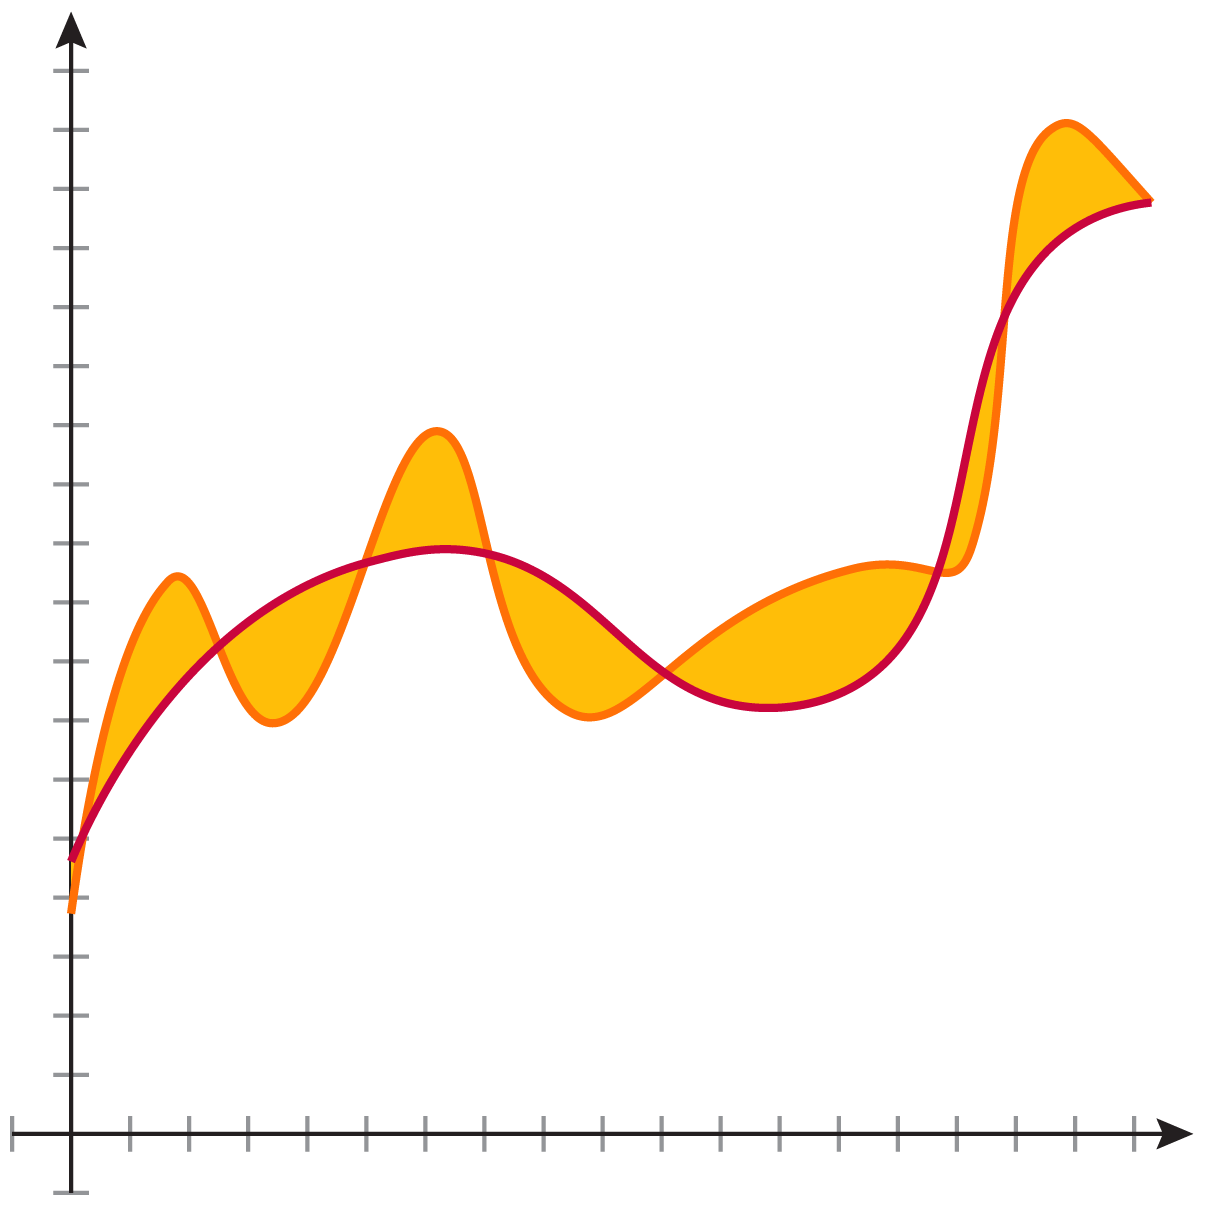
\includegraphics[width=\linewidth]{images/Rec1_FunctionNorms-02}
		\subcaption{$d_1$}
	\end{subfigure}
	\hspace{.1\linewidth}
	\begin{subfigure}[b]{.4\linewidth}
		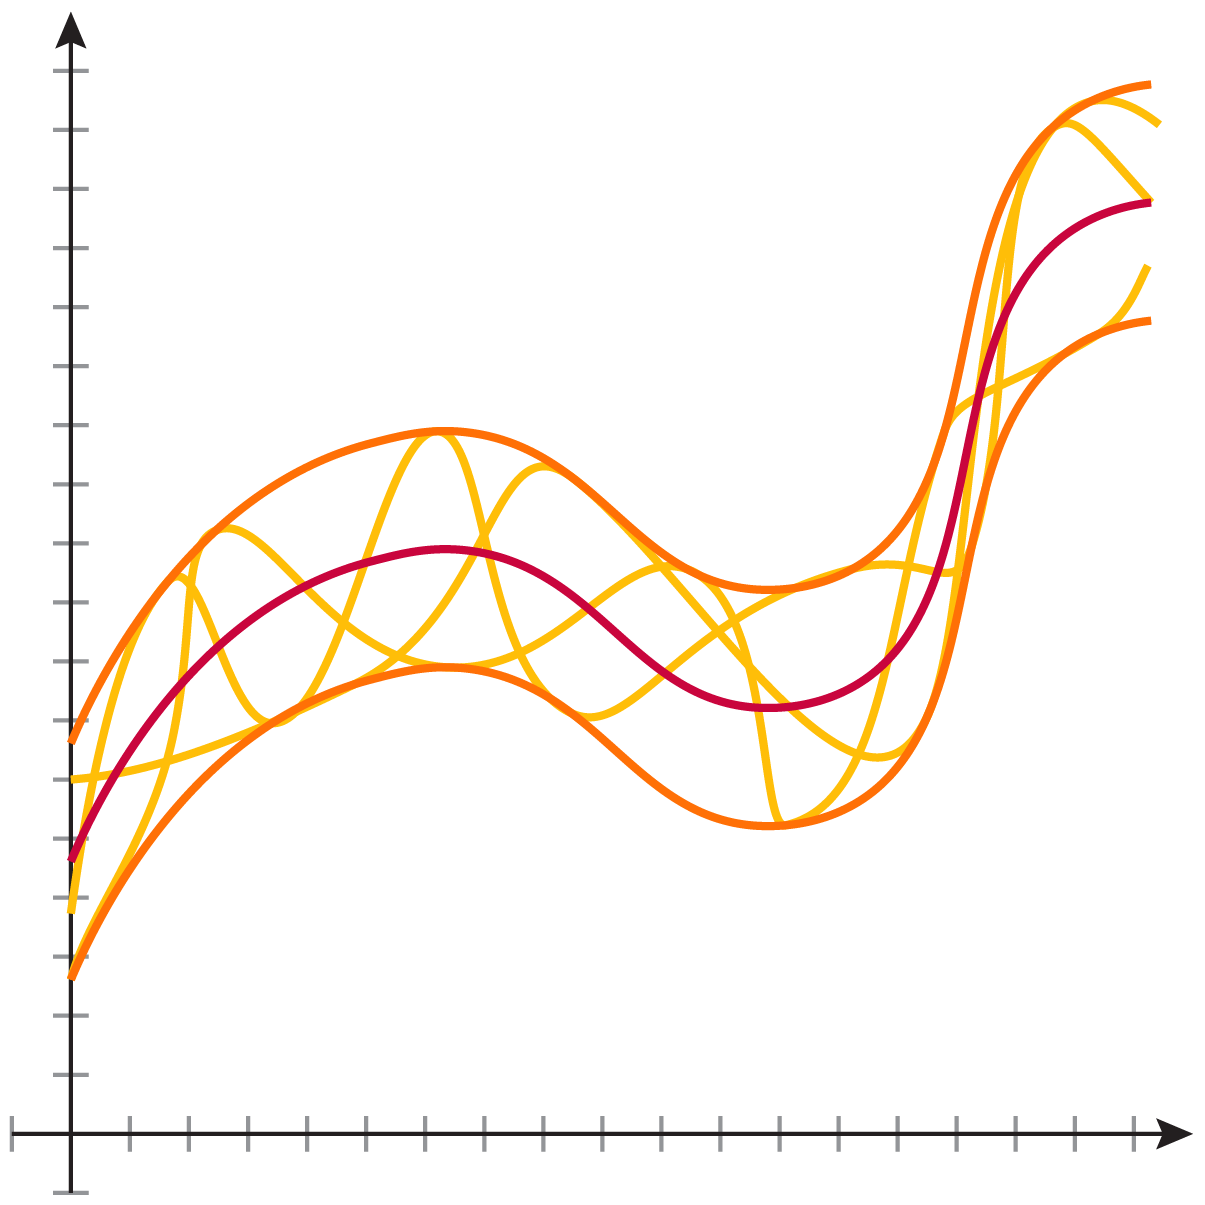
\includegraphics[width=\linewidth]{images/Rec1_FunctionNorms-01}
		\subcaption{$d_\infty$}
	\end{subfigure}
	\caption{spherical neighbourhoods in different distances on $\Cc^0$}
	\label{spherical-nbh-Cc0-different-distances}
\end{figure}

\paragraph{Metrics equivalence} What differences are there between a distance and another? Some times two distances are very ``similar'' each other:
\begin{defn} \label{equivalent-metrics}
	Let $X\neq \varnothing$ and $d$ and $\delta$ two different metrics on $X$.\\
	We say that $d$ and $\delta$ are \emph{equivalent} if there exist $c_1$ and $c_2>0$ such that:
	$$
	c_1\delta\left(x,y\right)
	\leq d\left(x,y\right)
	\leq c_2\delta\left(x,y\right) 
	\quad \forall x,y \in X$$
\end{defn}

Consider now two equivalent metrics, namely $d$ and $\delta$, observe that:
$$y \in B_d\left(x,y\right) \implies d\left(x,y\right) < r \implies \delta\left(x,y\right) < \frac r {c_1}$$
$$\implies y \in B_\delta \left(x,\frac r {c_1}\right) \qquad \forall x \in X \; \forall r > 0$$
In the same way we have: $y \in B_\delta\left(x,y\right) \implies y \in B_d \left(x,r\,c_2\right)$: the open balls with respect to $d$ and $\delta$, and of two equivalent metrics in general, are nested one inside another.

\begin{exam}
	Now we prove that $d_1, \, d_e, \, d_\infty$ on $\RR^N$ are equivalent:
	\begin{align*}
		d_\infty (x,y) &= \max_{k=1, \ldots, n} |x_k-y_k| = |x_{\bar{k}}-y_{\bar{k}}| \\
		&=\sqrt{\left(x_{\bar{k}} - y_{\bar{k}} \right)^2} \leq \sqrt{\sum_{k=1}^{n}\left(x_k-y_k\right)^2} =d_e\left(x,y\right)
	\end{align*}
	Now remember that if $a_1,\ldots,a_n\geq0$ then $a_1^2+\cdots+a_n^2\leq \left(a_1+\cdots+a_n\right)^2$:
	$$d_e \left(x,y\right) = \left(\sum_{k=1}^{n}\left(x_k-y_k\right)^2\right)^{\frac 1 2} \leq \left[ \left(\sum_{k=1}^{n}|x_k-y_k|\right)^2 \right]^{\frac 1 2} = d_1\left(x,y\right)$$
	Then we just need to prove that $d_1 \le c_1\,d_\infty$:
	$$d_1\left(x,y\right) = \sum_{k=1}^{n}|x_k-y_k| \leq \sum_{k=1}^{n} \max_{i=1, \ldots, n} |x_i-y_i| = n \cdot d_\infty\left(x,y\right)$$
	In the end we have $d_\infty(x, y) \le d_e(x, y) \le d_1(x, y) \le c_1 d_\infty(x, y)$, and the thesis is proven.
\end{exam} 

\begin{exam}
	The distances $d_1$ and $d_\infty$ on the space $\Cc^0([a, b])$ are \textit{not} equivalent. Indeed the distance $d_1$ can be controlled by the distance $d_\infty$:
	$$ d_1\left(f,g\right)=\int_{a}^{b}|f\left(x\right)-g\left(x\right)|\dx \leq \int_{a}^{b} d_\infty\left(f,g\right) \dx= d_\infty \left(f,g\right)\left(b-a\right)$$
	However $d_\infty$ cannot be controlled by $d_1$: let us prove that with a counterexample. Take $\left[a,b\right]=\left[0,1\right]$ and define $f_n$ as follows:
	$$f_n\left(x\right) = \begin{cases}
	n-n^2x & \text{if } x\in \left[0,\frac 1 n\right] \\
	0 & \text{if }x\in \left[\frac 1 n,1\right]
	\end{cases}$$
	\begin{figure}[htpb]
		\centering
		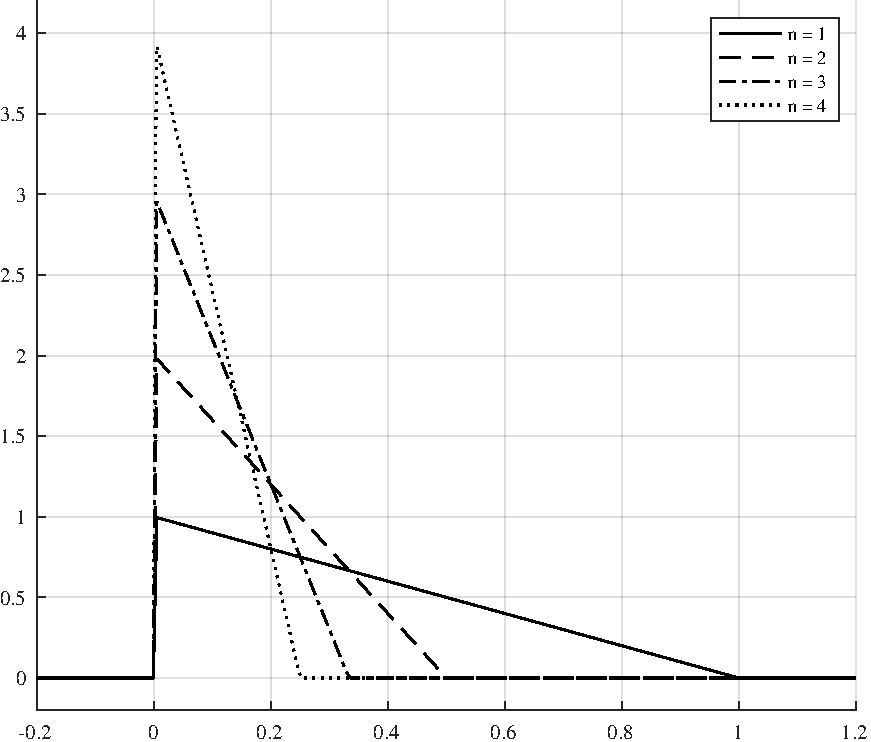
\includegraphics[width = 0.55\textwidth]{images/distances_not_equivalent}
	\end{figure}
	\FloatBarrier
	Then we have:
	$$
		d_1\left(f_n,0\right) 
		= \int_{0}^{\frac 1 n}\left(n-n^2x\right)\dx 
		= \left[nx-\frac{n^2x^2} 2\right]_0^\frac 1 n 
		= 1 - \frac 1 2 
		= \frac 1 2
	,
	$$
	and
	$$
		d_\infty(f_n, 0) 
		= n
	.
	$$
	Hence, there is no $c>0$ such that $d_\infty\left(f_n,0\right)\leq c\cdot d_1\left(f_n,0\right)$ for any $n$.
\end{exam}
